\documentclass[12pt]{article}
\usepackage[margin=3cm]{geometry}
\usepackage{graphicx}
\usepackage{float}

\begin{document}

\begin{titlepage}
	\begin{center}
		
		
		% Upper part of the page. The '~' is needed because \\
		% only works if a paragraph has started.
		\vfill
		
		\textsc{\LARGE Lab 2: Inverter Scehmatic}\\[1.5cm]
		
		\Large Adam Sumner\\[0.5cm]
		
		\Large Illinois Insititute of Technology\\[0.5cm]
		
		\Large ECE 429-01\\[0.5cm]	
		
		\noindent
		\vfill
		\large \textbf{Lab Date:} September 21\textsuperscript{st}, 2015\hfill
		\large \textbf{Due Date:} September 28\textsuperscript{th}, 2015
		% Bottom of the page
		
		
	\end{center}
\end{titlepage}

\section{Introduction}
The purpose of this lab is to introduce the student to the various tools that will be used throughout the semester. The student will design a schematic of a CMOS inverter, create the inverter in Virtuoso, and test the correctness of the design using HSPICE.

\section{Theory/Pre-Lab}
\subsection{Theory}
Due to the costly nature of manufacturing VLSI chips and the difficulty of testing devices on the nanoscale level, a majority of VLSI design work is done using computers and simulation  software. Designers rely heavily on CAD techniques to validate their designs before the designs are pushed into production. The Cadence Virtuoso platform is one of the most widely used commercial electronic design automation platform that supports custom IC designs. It serves as a central point for design entry, and it also provides various interfaces for use with other EDA tools. Throughout this lab, the FreePDK45 library, which supports a 45 nm process derived from the Predictive Technology Model, will be used.

Complementary MOSFET or CMOS technology is widely used in industry today. Devices ranging from Cell phones to CPU's all utilize CMOS due to its advantages over pure NMOS or pure PMOS designs. CMOS offers devices low power dissipation, relatively high speed, and high noise margins in both states. The most basic logic gate that can be implemented using CMOS is an inverter. This involves the use of only 2 MOSFETs, one PMOS type and one NMOS type. Figure \ref{fig:inverter} shows the layout of a CMOS inverter. 
\begin{figure}[H]
\centering
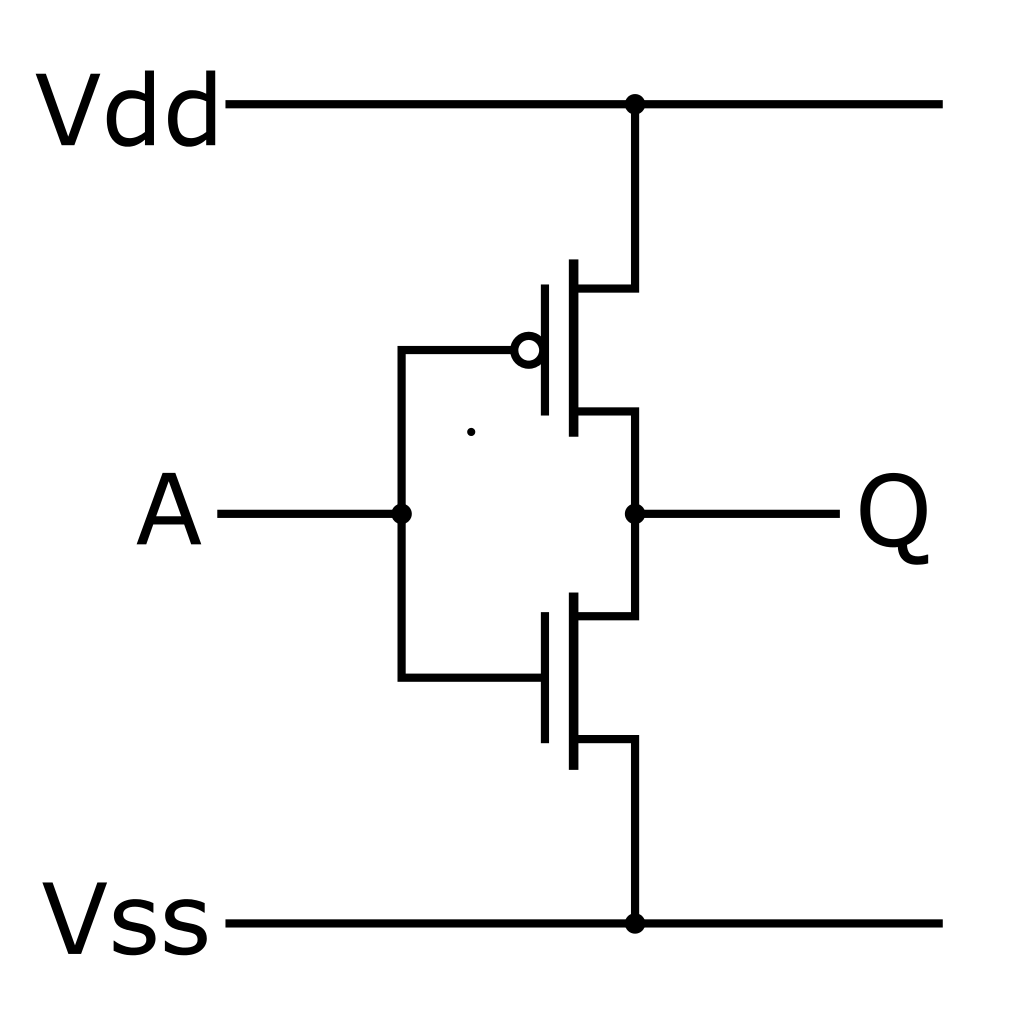
\includegraphics[width=0.4\linewidth]{inverter}
\caption{CMOS Inverter Schematic}
\label{fig:inverter}
\end{figure}


\subsection{Pre-Lab}
The pre-lab involved a refreshment of the various SPICE netlists, an overview of Tutorial I: Inverter Schematic and Simulation, and the creation of a schematic for a static CMOS inverter with power sources connected. The drawn schematic is shown below:
\begin{figure}[H]
\centering
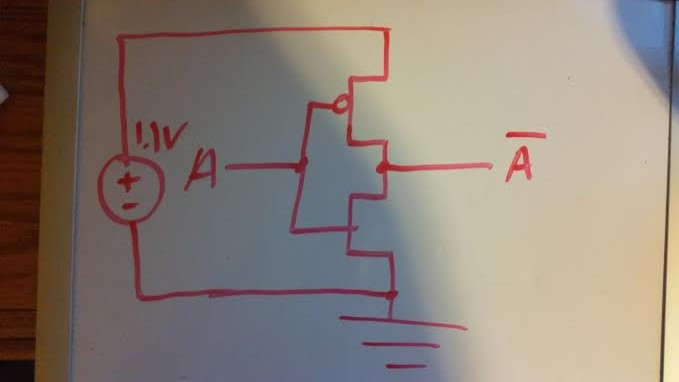
\includegraphics[width=1.0\linewidth]{prelab}
\caption{Static CMOS Inverter with Power Source}
\label{fig:prelab}
\end{figure}

\section{Implementation}

\section{Conclusions}

\end{document}
